\subsubsection{Minuta de reunião (24-Junho-2015)}

\begin{tabbing}
  Local \= xxx \kill
  Local \> : LEAD \\
  Data  \> : 24 de Junho de 2015 \\
  Hora  \> : 13:00
\end{tabbing}

%---------------------------------------------------------------------
\participantes{
  \elael,
  \gabriel,
  \julia,
  \renan,
  \alana,
  \estevão,
  \ramon.
}

\textbf{Aprovação da minuta}

\textbf{Update semanal do Projeto EMMA}
  
		
\textbf{\elael.} 
	\begin{itemize}
		\item \textbf{Tarefas concluídas:}
			\begin{itemize}    
				\item Análise do Shutter em andamento com novos números Rijeza.
				\item Análise de material de alta resistência. 
			\end{itemize}
		
		\item \textbf{Novas tarefas:}
			\begin{itemize} 
				\item SOTA: finalizar conceito para deadline de quarta-feira 
				\item Cerâmicas de compressão: descobrir o material que a Rijeza usa.
				\item Email Darlan: Informação sobre a chama e pistola de coating.
			\end{itemize}
	\end{itemize}
	
	\textbf{\renan.} 
	\begin{itemize}
		\item \textbf{Novas tarefas:}
			\begin{itemize} 
				\item Se unir a Gabriel para finalizar a workspace analysis.
				\item Formalizar conclusões no SOTA para deadline.
			\end{itemize}
	\end{itemize}
					
			
   \textbf{\gabriel.} 
	\begin{itemize}
		\item \textbf{Tarefas concluídas:}
			\begin{itemize}    
				\item Bugs no workspace analysis resolvidos.
				\item Análise motoman em andamento.
			\end{itemize}
		
		\item \textbf{Novas tarefas:}
			\begin{itemize} 
			    \item Manipuladores: Verificar modelo novo do motoman, 8 graus de
			    liberdade.
			    \item Resolver 'colisions issues' Open Rave.
				\item Adicionar conclusões no SOTA.
			\end{itemize}
	\end{itemize}
	
	   \textbf{\julia.} 
	\begin{itemize}
		\item \textbf{Tarefas concluídas:}
			\begin{itemize}    
				\item Apresentação
				\item Logo do Projeto EMMA
				\item Documentação de projeto atualizada.
			\end{itemize}
		
		\item \textbf{Novas tarefas:}
			\begin{itemize} 
			    \item Revisão Proposta com Patrick.
			    \item Apresentação EMMA. 
			    \item Cotações viagens.
			\end{itemize}
	\end{itemize}

  \textbf{\estevão.} 
	\begin{itemize}
		\item \textbf{Tarefas concluídas:}
			\begin{itemize}    
				\item Slides com SolidWorks da base para apresentação adicionados.
			\end{itemize}
		
		\item \textbf{Novas tarefas:}
			\begin{itemize} 
			    \item Continuar esboço do shutter.
			    \item Formalizar trabalho de mecânica no SOTA.
			\end{itemize}
	\end{itemize}
			



\textbf{Agenda para a próxima reunião:}
  \begin{itemize}
    \item Novas tarefas \& recomendações.
  \end{itemize}


\vspace{5mm}%
\parbox[t]{70mm}{
  Aprovado por: \\[5mm]
  \centering
  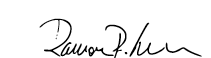
\includegraphics[width=65mm]{figs/logo/assinatura-ramon.png} \\[-4mm]
  \rule[2mm]{70mm}{0.1mm} \\
  \ramon \\[1mm]
  Coordenador do Projeto \\
}

%---------------------------------------------------------------------
\fim